\begin{ex}
Uma criança tem diante de si o desenho abaixo. Ela decidiu colorir apenas 4 dos 9 quadradinhos, um deles de vermelho e 3 de azul. De quantas maneiras diferentes essa pintura pode ser feita?
\begin{center}
 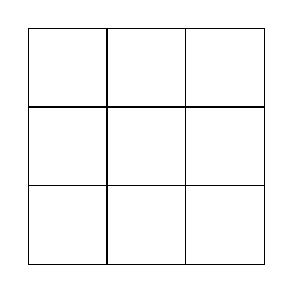
\begin{tikzpicture} 
 \draw (0,0)--(0,3)--(3,3)--(3,0)--(0,0);
 \draw (1,0)--(1,3);
 \draw (2,0)--(2,3);
 \draw (0,1)--(3,1);
 \draw (0,2)--(3,2);
 \end{tikzpicture}
\end{center}
  \begin{sol}
    \phantom{A} \\
    $9\cdot\mathrm{C}_{8,3}=504$
  \end{sol}

\end{ex}